\scanpage{158}
\margin{\textcircled{\unsure{d|e}}}
\deleted{Cela \unsure{par}}

On a donc trouvé un accouplement (\unsure{commutant|donnant} \unsure{à|:} la \unsure{permutation|multiplication} à un \unsure{signe})
\diagram{\begin{tikzcd}[ampersand replacement=\&,column sep=small,row sep=large]
\mathbb{R}\mathcal{H}om(\mathrm{pr}_1^*(F_\bullet),\mathrm{pr}_2^!(G_\bullet))\times\arrow[d,no head,bend left=25]
\&\mathbb{R}\mathcal{H}om(\mathrm{pr}_2^*(G_\bullet),\mathrm{pr}_1^!(F_\bullet))\arrow[r]\arrow[d,no head,bend left=35]
\&K_{X\times_S Y}^{\bullet}\\
\deleted{\text{D'où, pour }\xi^0\in\mathbb{R}^0\Gamma_{X\times_S Y}(\quad)}
\&\deleted{\text{et }\eta^0\in\mathbb{R}^0\Gamma_{X\times_S Y}(\quad)}\&
\end{tikzcd}}
\deleted{un élément $\unsure{\xi^0\cup\eta^0}$}
\deleted{$\xi^0\cup\eta^0\in\mathbb{R}^0\Gamma_{X\times_S Y}(K_{X\times_S Y}^{\bullet})$}

Appliquant $\mathbb{R}\Gamma_{X\times_S Y}$, on trouve un accouplement
\diagram{\begin{tikzcd}[ampersand replacement=\&,column sep=small]
\mathbb{R}\operatorname{Hom}^{\bullet}(\mathrm{pr}_1^*(F),\mathrm{pr}_2^!(G))\times \arrow[d,phantom,"\simeq" description]
\& \mathbb{R}\operatorname{Hom}^{\bullet}(\mathrm{pr}_2^*(G),\mathrm{pr}_1^!(F)) \arrow[r] \arrow[d,phantom,"\simeq" description]
\& \mathbb{R}\Gamma_{X\times_S Y}K_{X\times_S Y}^{\bullet}\arrow[d]\\
\mathbb{R}\operatorname{Hom}^{\bullet}(\unsure{\mathbb{R}f_*}(F),\unsure{\mathbb{R}g_*}(G))\times
\& \mathbb{R}\operatorname{Hom}^{\bullet}(\unsure{\mathbb{R}g_*}(G),\unsure{\mathbb{R}f_*}(F))\arrow[r]
\& \deleted{\unsure{\mathbb{R}}}A_S
\end{tikzcd}}
qui ne doit être autre que l'accouplement déjà connu \unsure{relatif} ; $P_\bullet\simeq\unsure{\mathrm{pr}_{1*}|\mathbb{R}f_*}(F_\bullet)$ et $Q_\bullet\simeq\unsure{\mathrm{pr}_{2*}|\mathbb{R}g_*}(G_\bullet)$.

En particulier, si
\[
\xi^0\in\mathbb{R}^0\operatorname{Hom}^{\bullet}(\mathrm{pr}_1^*(\unsure{P|F}),\mathrm{pr}_2^!(\unsure{Q|G}))
=\mathbb{R}^0\Gamma_{X\times_S Y}\,\mathbb{R}\mathcal{H}om(\mathrm{pr}_1^*(F),\mathrm{pr}_2^!(G_\bullet))
\]
\[
\eta^0\in\mathbb{R}^0\operatorname{Hom}^{\bullet}(\mathrm{pr}_2^*(\unsure{Q|G}),\mathrm{pr}_1^!(F))
=\mathbb{R}^0\Gamma_{X\times_S Y}\,\mathbb{R}\mathcal{H}om(\mathrm{pr}_1^*(F),\mathrm{pr}_2^!(G_\bullet))
\]
alors
\[
\xi^0\cup\eta^0\in\mathbb{R}^0\Gamma_{X\times_S Y}(K_{X\times_S Y}^{\bullet})\xrightarrow{\operatorname{Tr}_h} A.
\]
et on aura
\[
\boxed{\operatorname{Tr}(\xi^0\cup\eta^0)=\langle\xi^0,\eta^0\rangle}
\qquad
\left(=\sum_i\operatorname{Tr}(\xi^0)^{(i)}(\eta^0)^{(\unsure{-i|i})}\unsure{(-1)^i}\right)
\]
\figure{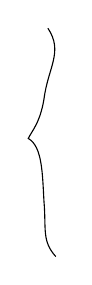
\begin{tikzpicture}[x=1cm,y=1cm]
\draw (.25,1.4)..controls(.45,1.1) and (.25,.9)..(.2,.5)..controls(.15,.2) and (.05,.1)..(0,0)..controls(.18,-.1) and (.18,-.45)..(.2,-.8)..controls(.23,-1.15) and (.17,-1.3)..(.35,-1.5);
\end{tikzpicture}}
\margin{si on représente $\unsure{f_*}(P),\unsure{g_*}(Q)$ par des complexes plats de type fini en chaque degré !).}
\margin{157}
